\documentclass[aspectratio=169,10pt]{beamer}

\usetheme{default}
\usecolortheme{default}
\usefonttheme{professionalfonts}
\usepackage[T1]{fontenc}
\usepackage{ebgaramond}
\usepackage[scale=0.94]{tgheros}
\usepackage{amsmath,amssymb,mathtools,booktabs,graphicx,array,tikz}
\usepackage{appendixnumberbeamer}
\usetikzlibrary{arrows.meta,positioning,shapes.geometric}
\usepackage[backend=biber,style=numeric,sorting=none,maxbibnames=3]{biblatex}
\addbibresource{../../../../research-monograph/references.bib}

% De La Salle presentation palette.
\definecolor{dlsugreen}{RGB}{0,129,77}
\definecolor{dlsudarkgreen}{RGB}{0,82,49}
\definecolor{dlsupalegreen}{RGB}{235,246,240}
\definecolor{charcoal}{RGB}{34,43,46}
\definecolor{midgray}{RGB}{96,108,111}
\definecolor{lightgray}{RGB}{244,246,245}
\definecolor{resultblue}{RGB}{31,86,135}
\definecolor{cautionred}{RGB}{166,27,41}
\definecolor{warmgold}{RGB}{180,116,0}

\setbeamercolor{normal text}{fg=charcoal,bg=white}
\setbeamercolor{structure}{fg=dlsugreen}
\setbeamercolor{alerted text}{fg=cautionred}
\setbeamercolor{frametitle}{fg=dlsudarkgreen,bg=white}
\setbeamercolor{frametitle rule}{bg=dlsugreen}
\setbeamercolor{title}{fg=white}
\setbeamercolor{subtitle}{fg=white!90}
\setbeamercolor{author}{fg=white}
\setbeamercolor{institute}{fg=white!88}
\setbeamercolor{date}{fg=white!78}
\setbeamercolor{block title}{fg=white,bg=dlsugreen}
\setbeamercolor{block body}{fg=charcoal,bg=dlsupalegreen}
\setbeamercolor{block title example}{fg=white,bg=resultblue}
\setbeamercolor{block body example}{fg=charcoal,bg=resultblue!7}
\setbeamercolor{block title alerted}{fg=white,bg=cautionred}
\setbeamercolor{block body alerted}{fg=charcoal,bg=cautionred!7}
\setbeamercolor{author in head/foot}{fg=midgray,bg=white}
\setbeamercolor{date in head/foot}{fg=white,bg=dlsugreen}

\setbeamerfont{title}{family=\rmfamily,series=\bfseries,size=\fontsize{24}{26}}
\setbeamerfont{subtitle}{family=\sffamily,series=\bfseries,size=\fontsize{13}{16}}
\setbeamerfont{author}{family=\sffamily,series=\bfseries,size=\normalsize}
\setbeamerfont{institute}{family=\sffamily,size=\small}
\setbeamerfont{date}{family=\sffamily,size=\footnotesize}
\setbeamerfont{frametitle}{family=\sffamily,series=\bfseries,size=\fontsize{16}{18}}
\setbeamerfont{block title}{family=\sffamily,series=\bfseries}
\setbeamerfont{footline}{family=\sffamily,size=\fontsize{6.8}{8}}

\setbeamertemplate{navigation symbols}{}
\setbeamertemplate{blocks}[rounded][shadow=false]
\setbeamertemplate{itemize item}{\raise0.15ex\hbox{\small\textbullet}}
\setbeamertemplate{itemize subitem}{\raise0.15ex\hbox{\scriptsize\textbullet}}
\setbeamertemplate{enumerate item}{\insertenumlabel.}
\setbeamersize{text margin left=0.55cm,text margin right=0.55cm}

\setbeamertemplate{frametitle}{%
  \nointerlineskip
  \begin{beamercolorbox}[wd=\paperwidth,ht=0.66cm,dp=0.18cm,leftskip=0.55cm,rightskip=0.45cm]{frametitle}
    \usebeamerfont{frametitle}\insertframetitle
  \end{beamercolorbox}%
  \begin{beamercolorbox}[wd=\paperwidth,ht=0.035cm]{frametitle rule}\end{beamercolorbox}%
}

\setbeamertemplate{footline}{%
  \leavevmode
  \hbox{%
    \begin{beamercolorbox}[wd=.84\paperwidth,ht=2.8ex,dp=1.15ex,leftskip=.45cm]{author in head/foot}%
      \textbf{\textcolor{dlsugreen}{DE LA SALLE UNIVERSITY}}%
      \hspace{0.65em}\textcolor{midgray!50}{|}\hspace{0.65em}\insertshorttitle
    \end{beamercolorbox}%
    \begin{beamercolorbox}[wd=.16\paperwidth,ht=2.8ex,dp=1.15ex,center]{date in head/foot}%
      \insertframenumber\,/\,\inserttotalframenumber
    \end{beamercolorbox}%
  }%
}

\hypersetup{colorlinks=true,linkcolor=dlsugreen,urlcolor=dlsugreen,citecolor=resultblue}
\pdfstringdefDisableCommands{\def\translate#1{#1}}

\newcommand{\Eref}{E_{\mathrm{ref}}}
\newcommand{\norm}[1]{\left\lVert#1\right\rVert}
\newcommand{\calcroot}{../../../../../../calculations}
\newcommand{\takeaway}[1]{%
  \begin{beamercolorbox}[rounded=true,sep=0.55em,wd=\textwidth]{block body example}
    \centering\large\bfseries\color{resultblue}#1
  \end{beamercolorbox}}
\newcommand{\boundary}[1]{\textcolor{cautionred}{\textbf{Boundary:}} #1}

\title[Compatibility of spectral and operator reductions]{Compatibility of Spectral and Operator Reductions of a First-Principles Silicon Hamiltonian}
\subtitle{Exact rank-two compatibility geometry and a rank-10 silicon Wannier case study}
\author{Eugene Joseph M. Ragasa}
\institute{De La Salle University, Department of Physics\\
\href{mailto:eugene.ragasa@dlsu.edu.ph}{\textcolor{white!88}{eugene.ragasa@dlsu.edu.ph}}}
\date{\textbf{4th International Conference on Materials Science and Engineering\\
in the Philippines (ICMSEP 2026)}\\
5--7 November 2026 $\cdot$ Widus Hotel, Clark, Pampanga, Philippines}

\begin{document}

{
\setbeamercolor{background canvas}{bg=dlsugreen}
\setbeamertemplate{footline}{}
\begin{frame}[plain]
  \vfill
  
\includegraphics[width=.30\paperwidth]{assets/dlsu-wordmark-white.png}\par
  \vspace{0.5em}
  {\usebeamerfont{title}\usebeamercolor[fg]{title}\inserttitle\par}
  \vspace{0.25em}
  {\color{white!55}\rule{.20\paperwidth}{0.8pt}\par}
  \vspace{0.35em}
  {\usebeamerfont{subtitle}\usebeamercolor[fg]{subtitle}\insertsubtitle\par}
  \vspace{0.6em}
  {\usebeamerfont{author}\usebeamercolor[fg]{author}\insertauthor\par}
  \vspace{0.15em}
  {\usebeamerfont{institute}\usebeamercolor[fg]{institute}\insertinstitute\par}
  \vspace{0.4em}
  {\usebeamerfont{date}\usebeamercolor[fg]{date}\insertdate\par}
  \vfill
\end{frame}
}

\section{Introduction}
{
\setbeamercolor{background canvas}{bg=dlsugreen}
\setbeamertemplate{footline}{}
\begin{frame}[plain]
  \centering
  \vfill
  
\includegraphics[width=.23\paperwidth]{assets/dlsu-wordmark-white.png}\par
  \vspace{0.8em}
  {\sffamily\bfseries\large\color{white!65}SECTION I\par}
  \vspace{0.25em}
  {\sffamily\bfseries\fontsize{30}{34}\selectfont\color{white}Introduction\par}
  \vspace{0.4em}
  {\sffamily\large\color{white!85}
  Representations, retained subspaces, and finite-range cost\par}
  \vfill
\end{frame}
}

\begin{frame}{The time-independent Schrödinger equation}
  \small
  \begin{beamercolorbox}[rounded=true,sep=0.55em,wd=\textwidth]{block body example}
    \centering\Large\bfseries\color{resultblue}
    $\hat H\lvert\psi_n\rangle=E_n\lvert\psi_n\rangle$
  \end{beamercolorbox}
  \vspace{0.6em}
  \begin{columns}[T]
    \column{0.47\textwidth}
      \begin{block}{Spectral representation}
        In a finite-dimensional numerical representation,
        \[
          \hat H=\sum_n E_n
          \lvert\psi_n\rangle\langle\psi_n\rvert.
        \]
        The operator is represented by its eigenvalues and eigenvectors.
      \end{block}
    \column{0.47\textwidth}
      \begin{exampleblock}{Real-space representation}
        \[
          H(\mathbf r,\mathbf r')
          =\langle\mathbf r\rvert\hat H\lvert\mathbf r'\rangle,
        \]
        \[
          \int H(\mathbf r,\mathbf r')\psi_n(\mathbf r')\,d\mathbf r'
          =E_n\psi_n(\mathbf r).
        \]
        The same operator is represented as a coordinate-space kernel.
      \end{exampleblock}
  \end{columns}
  \vspace{0.35em}
  \centering\textbf{The spectrum and the real-space matrix describe the same operator,
  but they expose different information.}
\end{frame}

\begin{frame}{From full reconstruction to a retained subspace}
  \small
  \begin{columns}[T]
    \column{0.51\textwidth}
      \begin{block}{Full and rank-$N$ reconstruction}
        \[
          \hat H_M=\sum_{n=1}^{M}E_n
          \lvert\psi_n\rangle\langle\psi_n\rvert,
        \]
        \[
          \begin{aligned}
            P_N&=\sum_{n\in\mathcal W}
            \lvert\psi_n\rangle\langle\psi_n\rvert,\\
            \hat H_N&=P_N\hat H_M P_N,\qquad N<M.
          \end{aligned}
        \]
      \end{block}
    \column{0.45\textwidth}
      \begin{exampleblock}{Rank $N<M$}
        \begin{itemize}
          \setlength{\itemsep}{0.15em}
          \item the DFT--PAW parent can be high dimensional;
          \item the target may occupy a frontier-band window; and
          \item a retained rank-$N$ model can make interpolation and downstream
            analysis more tractable.
        \end{itemize}
        Projection remains a separate approximation that must be assessed.
      \end{exampleblock}
  \end{columns}
  \vspace{0.55em}
  \centering
  {\large\bfseries\color{dlsudarkgreen}
  From the retained periodic subspace to hopping blocks\par}
  \vspace{0.35em}
  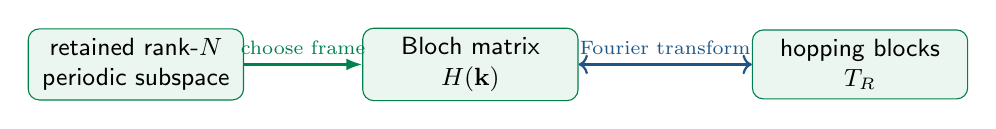
\begin{tikzpicture}[
      every node/.style={font=\sffamily\small,align=center},
      box/.style={draw=dlsugreen,rounded corners,fill=dlsupalegreen,minimum height=0.72cm,text width=2.5cm},
      arrow/.style={-{Latex[length=2mm]},thick,dlsugreen}]
    \node[box] (subspace) {retained rank-$N$\\periodic subspace};
    \node[box,right=1.5cm of subspace] (bloch) {Bloch matrix\\$H(\mathbf k)$};
    \node[box,right=2.2cm of bloch] (hopping) {hopping blocks\\$T_R$};
    \draw[arrow] (subspace) -- node[above,font=\scriptsize] {choose frame} (bloch);
    \draw[<->,thick,resultblue] (bloch) -- node[above,font=\scriptsize] {Fourier transform} (hopping);
  \end{tikzpicture}
\end{frame}

\begin{frame}{The model: matrix-valued hoppings between cells}
  \small
  \begin{columns}[T]
    \column{0.48\textwidth}
      \centering
      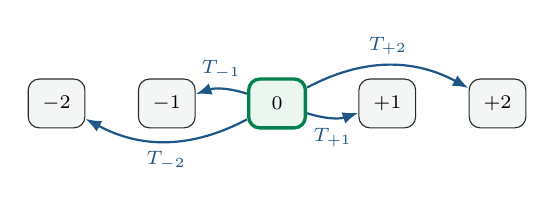
\begin{tikzpicture}[
          cell/.style={draw=charcoal,rounded corners,minimum width=0.72cm,minimum height=0.62cm,fill=lightgray,font=\sffamily\scriptsize},
          home/.style={cell,draw=dlsugreen,very thick,fill=dlsupalegreen},
          hop/.style={-{Latex[length=2mm]},thick,resultblue}]
        \node[cell] (m2) at (-2.8,0) {$-2$};
        \node[cell] (m1) at (-1.4,0) {$-1$};
        \node[home] (z) at (0,0) {$0$};
        \node[cell] (p1) at (1.4,0) {$+1$};
        \node[cell] (p2) at (2.8,0) {$+2$};
        \draw[hop] (z) to[bend right=18] node[below,font=\scriptsize] {$T_{+1}$} (p1);
        \draw[hop] (z) to[bend left=28] node[above,font=\scriptsize] {$T_{+2}$} (p2);
        \draw[hop] (z) to[bend right=18] node[above,font=\scriptsize] {$T_{-1}$} (m1);
        \draw[hop] (z) to[bend left=28] node[below,font=\scriptsize] {$T_{-2}$} (m2);
      \end{tikzpicture}
    \column{0.48\textwidth}
      \begin{block}{Hopping block $T_R$}
        A matrix coupling the retained orbital coordinates in cell $0$ to those in cell
        $R$. Hermiticity requires $T_{-R}=T_R^\dagger$.
      \end{block}
  \end{columns}
  \vspace{0.55em}
  \begin{columns}[T]
    \column{0.47\textwidth}
      \begin{exampleblock}{Complete periodic model}
        \[
          H(\mathbf k)=\sum_R T_R e^{i\mathbf k\cdot R}.
        \]
        All hopping blocks contribute to the complete Bloch Hamiltonian.
      \end{exampleblock}
    \column{0.47\textwidth}
      \begin{block}{Finite-range reduction}
        \[
          H^{(R_c)}(\mathbf k)
          =\sum_{|R|\le R_c}T_R e^{i\mathbf k\cdot R}.
        \]
        Increasing $R_c$ retains more real-space information and usually lowers the
        truncation error.
      \end{block}
  \end{columns}
  \vspace{0.2em}
  \begin{beamercolorbox}[rounded=true,sep=0.45em,wd=\textwidth]{block body example}
    \centering\bfseries\color{resultblue}
    At a fixed error target, the range cost is the smallest sampled cutoff $R_c$ for
    which the truncated model passes.
  \end{beamercolorbox}
\end{frame}

\section{Scientific software implementation}
{
\setbeamercolor{background canvas}{bg=dlsugreen}
\setbeamertemplate{footline}{}
\begin{frame}[plain]
  \centering
  \vfill
  
\includegraphics[width=.23\paperwidth]{assets/dlsu-wordmark-white.png}\par
  \vspace{0.8em}
  {\sffamily\bfseries\large\color{white!65}SECTION II\par}
  \vspace{0.25em}
  {\sffamily\bfseries\fontsize{30}{34}\selectfont\color{white}
  Scientific Software Implementation\par}
  \vspace{0.4em}
  {\sffamily\large\color{white!85}
  Strong types, formal checks, and operator-guided LLM development\par}
  \vfill
\end{frame}
}

\begin{frame}{Spectral and spatial reductions in a common fit basis}
  \centering
  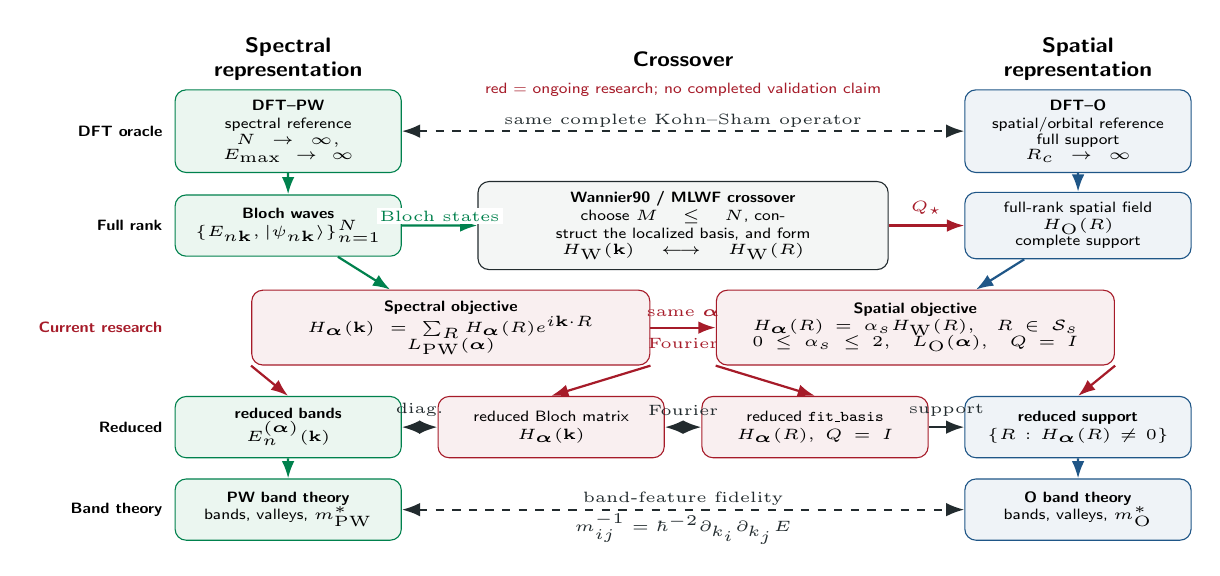
\begin{tikzpicture}[
      xscale=1.18,
      yscale=1.08,
      transform shape,
      >=Latex,
      every node/.style={font=\sffamily\tiny,align=center},
      greenbox/.style={draw=dlsugreen,rounded corners,fill=dlsupalegreen,
        minimum height=0.72cm,text width=2.20cm},
      bluebox/.style={draw=resultblue,rounded corners,fill=resultblue!7,
        minimum height=0.72cm,text width=2.20cm},
      graybox/.style={draw=charcoal,rounded corners,fill=lightgray,
        minimum height=0.72cm,text width=2.20cm},
      redbox/.style={draw=cautionred,rounded corners,fill=cautionred!7,
        minimum height=0.88cm,text width=4.05cm},
      greenflow/.style={-{Latex[length=2.2mm,width=1.6mm]},thick,dlsugreen},
      blueflow/.style={-{Latex[length=2.2mm,width=1.6mm]},thick,resultblue},
      redflow/.style={-{Latex[length=2.2mm,width=1.6mm]},thick,cautionred}]

    \node[font=\sffamily\scriptsize\bfseries] at (-4.25,2.78)
      {Spectral\\representation};
    \node[font=\sffamily\scriptsize\bfseries] at (0,2.78) {Crossover};
    \node[font=\sffamily\scriptsize\bfseries] at (4.25,2.78)
      {Spatial\\representation};
    \node[font=\sffamily\tiny\color{cautionred}] at (0,2.42)
      {red = ongoing research; no completed validation claim};

    \node[anchor=east,font=\sffamily\tiny\bfseries] at (-5.48,1.93) {DFT oracle};
    \node[anchor=east,font=\sffamily\tiny\bfseries] at (-5.48,0.82) {Full rank};
    \node[anchor=east,font=\sffamily\tiny\bfseries\color{cautionred}]
      at (-5.48,-0.38) {Current research};
    \node[anchor=east,font=\sffamily\tiny\bfseries] at (-5.48,-1.55) {Reduced};
    \node[anchor=east,font=\sffamily\tiny\bfseries] at (-5.48,-2.52) {Band theory};

    \node[greenbox,minimum height=0.92cm] (dftpw) at (-4.25,1.93) {
      \textbf{DFT--PW}\\
      spectral reference\\[-0.08em]
      $N\rightarrow\infty,$\\[-0.20em]
      $E_{\max}\rightarrow\infty$
    };
    \node[bluebox,minimum height=0.92cm] (dfto) at (4.25,1.93) {
      \textbf{DFT--O}\\
      spatial/orbital reference\\[-0.08em]
      full support\\[-0.20em]
      $R_c\rightarrow\infty$
    };
    \draw[<->,dashed,thick,charcoal] (dftpw.east) --
      node[above,font=\tiny,fill=white,inner sep=1pt]
      {same complete Kohn--Sham operator} (dfto.west);

    \node[greenbox] (bloch) at (-4.25,0.82) {
      \textbf{Bloch waves}\\[-0.05em]
      $\{E_{n\mathbf k},\lvert\psi_{n\mathbf k}\rangle\}_{n=1}^{N}$
    };
    \node[graybox,text width=4.18cm,minimum height=0.96cm] (wannier) at (0,0.82) {
      \textbf{Wannier90 / MLWF crossover}\\
      choose $M\leq N$, construct the localized basis, and form\\[-0.12em]
      $H_{\mathrm W}(\mathbf k)\ \longleftrightarrow\ H_{\mathrm W}(R)$
    };
    \node[bluebox] (fullspatial) at (4.25,0.82) {
      full-rank spatial field\\[-0.05em]
      $H_{\mathrm O}(R)$\\[-0.12em]
      complete support
    };
    \draw[greenflow] (dftpw) -- (bloch);
    \draw[greenflow] (bloch) --
      node[above,font=\tiny,fill=white,inner sep=1pt] {Bloch states} (wannier);
    \draw[blueflow] (dfto) -- (fullspatial);
    \draw[<->,redflow] (wannier.east) --
      node[above,font=\tiny\color{cautionred}] {$Q_\star$} (fullspatial.west);

    \node[redbox] (specobj) at (-2.50,-0.38) {
      \textbf{Spectral objective}\\[-0.06em]
      $H_{\boldsymbol\alpha}(\mathbf k)
       =\sum_R H_{\boldsymbol\alpha}(R)e^{i\mathbf k\cdot R}$\\[-0.10em]
      $L_{\mathrm{PW}}(\boldsymbol\alpha)$
    };
    \node[redbox] (opobj) at (2.50,-0.38) {
      \textbf{Spatial objective}\\[-0.06em]
      $H_{\boldsymbol\alpha}(R)=\alpha_sH_{\mathrm W}(R),\quad R\in\mathcal S_s$\\[-0.10em]
      $0\leq\alpha_s\leq2,\quad L_{\mathrm O}(\boldsymbol\alpha),\quad Q=I$
    };
    \draw[greenflow] (bloch) -- (specobj);
    \draw[blueflow] (fullspatial) -- (opobj);
    \draw[<->,redflow] (specobj.east) --
      node[above,font=\tiny\color{cautionred}] {same $\boldsymbol\alpha$}
      node[below,font=\tiny\color{cautionred}] {Fourier} (opobj.west);

    \node[greenbox] (redbands) at (-4.25,-1.55) {
      \textbf{reduced bands}\\[-0.04em]
      $E_n^{(\boldsymbol\alpha)}(\mathbf k)$
    };
    \node[graybox,draw=cautionred,fill=cautionred!7] (redbloch) at (-1.42,-1.55) {
      reduced Bloch matrix\\[-0.04em]
      $H_{\boldsymbol\alpha}(\mathbf k)$
    };
    \node[graybox,draw=cautionred,fill=cautionred!7] (redfit) at (1.42,-1.55) {
      reduced \texttt{fit\_basis}\\[-0.04em]
      $H_{\boldsymbol\alpha}(R),\ Q=I$
    };
    \node[bluebox] (redsupport) at (4.25,-1.55) {
      \textbf{reduced support}\\[-0.04em]
      $\{R:H_{\boldsymbol\alpha}(R)\ne0\}$
    };
    \draw[redflow] (specobj.south west) -- (redbands.north);
    \draw[redflow] (specobj.south east) -- (redbloch.north);
    \draw[redflow] (opobj.south west) -- (redfit.north);
    \draw[redflow] (opobj.south east) -- (redsupport.north);
    \draw[<->,thick,charcoal] (redbands.east) --
      node[above,font=\tiny] {diag.} (redbloch.west);
    \draw[<->,thick,charcoal] (redbloch.east) --
      node[above,font=\tiny] {Fourier} (redfit.west);
    \draw[->,thick,charcoal] (redfit.east) --
      node[above,font=\tiny] {support} (redsupport.west);

    \node[greenbox] (pwtheory) at (-4.25,-2.52) {
      \textbf{PW band theory}\\[-0.04em]
      bands, valleys, $m^*_{\mathrm{PW}}$
    };
    \node[bluebox] (otheory) at (4.25,-2.52) {
      \textbf{O band theory}\\[-0.04em]
      bands, valleys, $m^*_{\mathrm O}$
    };
    \draw[greenflow] (redbands) -- (pwtheory);
    \draw[blueflow] (redsupport) -- (otheory);
    \draw[<->,dashed,thick,charcoal] (pwtheory.east) --
      node[above,font=\tiny,fill=white,inner sep=1pt] {band-feature fidelity}
      node[below,font=\tiny,fill=white,inner sep=1pt]
      {$m_{ij}^{-1}=\hbar^{-2}\partial_{k_i}\partial_{k_j}E$}
      (otheory.west);
  \end{tikzpicture}
\end{frame}

\begin{frame}{Research background and implementation capabilities}
  \begin{columns}[T,onlytextwidth]
    \column{0.47\textwidth}
      \begin{block}{Education}
        \scriptsize
        \begin{itemize}\setlength{\itemsep}{0.12em}
          \item BS Mathematics and BS Economics, U.S. Military Academy, West Point;
          \item MA Mathematics, specialization in Mathematical Finance,
            Columbia University;
          \item MSES Mechanical Engineer, U. Pacific;
          \item PhD Materials Science and Engineering, U. Florida.
        \end{itemize}
      \end{block}
      \begin{exampleblock}{Experience and research}
        \scriptsize
        \begin{itemize}\setlength{\itemsep}{0.12em}
          \item computer consultant: network design, optimization, and deployment;
          \item quantitative analyst;
          \item master's research: viscoelastic materials and long-term stress--strain prediction;
          \item PhD research: DFT, molecular dynamics, potential development, and lattice dynamics.
        \end{itemize}
      \end{exampleblock}
    \column{0.50\textwidth}
      \begin{block}{Skills mapped into this program}
        \scriptsize
        \begin{tabular}{@{}p{0.34\linewidth}p{0.59\linewidth}@{}}
          \textbf{Mathematics} & compatibility geometry, proofs, Lean \\[0.25em]
          \textbf{Quantitative analysis} & optimization, model selection, diagnostics \\[0.25em]
          \textbf{Computing systems} & architecture, tools, deployment, provenance \\[0.25em]
          \textbf{Mechanics} & constitutive behavior and reduced models \\[0.25em]
          \textbf{Materials science} & DFT, Wannier, MD, potentials, phonons
        \end{tabular}
      \end{block}
      \begin{alertblock}{Minimum one-person capability}
        \scriptsize
        Domain physics, mathematics, numerics, software engineering, formal/software
        verification, provenance, and scientific judgment must remain connected. The
        LLM accelerates implementation; it does not replace expertise, review, or
        scientific authority.
      \end{alertblock}
  \end{columns}
\end{frame}

\begin{frame}{Implementation scale: scientific software stack}
  \centering
  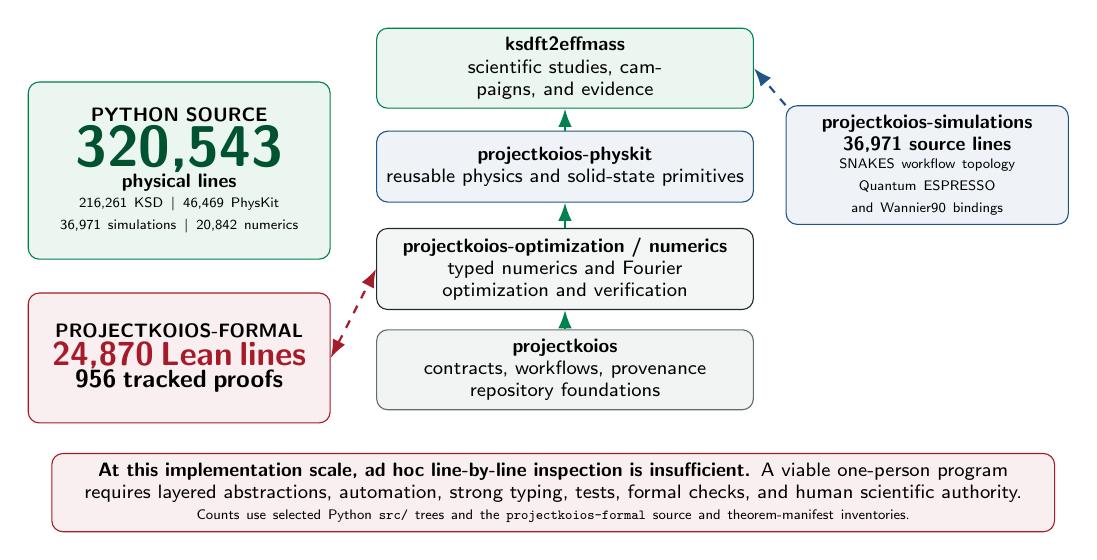
\begin{tikzpicture}[
      >=Latex,
      every node/.style={font=\sffamily\scriptsize,align=center},
      layer/.style={rounded corners,minimum height=0.90cm,text width=4.55cm},
      simulation/.style={rounded corners,minimum height=1.35cm,text width=3.35cm},
      metric/.style={rounded corners,text width=3.6cm},
      flow/.style={->,thick,dlsugreen},
      handoff/.style={->,dashed,thick,resultblue}]
    \node[metric,draw=dlsugreen,fill=dlsupalegreen,minimum height=2.25cm]
      (pythonmetric) at (-4.75,1.10) {
      \textbf{PYTHON SOURCE}\\[0.12em]
      {\fontsize{21}{23}\selectfont\bfseries\color{dlsudarkgreen}320,543}\\[-0.05em]
      \textbf{physical lines}\\[0.18em]
      {\tiny 216,261 KSD $\mid$ 46,469 PhysKit\\36,971 simulations $\mid$ 20,842 numerics}
    };
    \node[metric,draw=cautionred,fill=cautionred!7,minimum height=1.65cm]
      (lean) at (-4.75,-1.28) {
      \textbf{PROJECTKOIOS-FORMAL}\\[0.10em]
      {\large\bfseries\color{cautionred}24,870 Lean lines}\\
      {\small\bfseries 956 tracked proofs}
    };

    \node[layer,draw=dlsugreen,fill=dlsupalegreen] (ksd) at (0.15,2.40) {
      \textbf{ksdft2effmass}\\
      scientific studies, campaigns, and evidence
    };
    \node[layer,draw=resultblue,fill=resultblue!7] (physkit) at (0.15,1.15) {
      \textbf{projectkoios-physkit}\\
      reusable physics and solid-state primitives
    };
    \node[layer,draw=charcoal,fill=lightgray] (numerics) at (0.15,-0.15) {
      \textbf{projectkoios-optimization / numerics}\\
      typed numerics and Fourier\\optimization and verification
    };
    \node[layer,draw=midgray,fill=midgray!8] (core) at (0.15,-1.43) {
      \textbf{projectkoios}\\
      contracts, workflows, provenance\\repository foundations
    };
    \node[simulation,draw=resultblue,fill=resultblue!7] (simulations) at (4.75,1.17) {
      \textbf{projectkoios-simulations}\\
      {\bfseries 36,971 source lines}\\[0.05em]
      {\tiny SNAKES workflow topology\\Quantum ESPRESSO and Wannier90 bindings}
    };

    \draw[flow] (core) -- (numerics);
    \draw[flow] (numerics) -- (physkit);
    \draw[flow] (physkit) -- (ksd);
    \draw[handoff] (simulations.north west) -- (ksd.east);
    \draw[<->,dashed,thick,cautionred] (lean.east) -- (numerics.west);

    \node[draw=cautionred,rounded corners,fill=cautionred!7,
      font=\sffamily\scriptsize,text width=12.5cm,minimum height=0.86cm] at (0,-2.99) {
      \textbf{At this implementation scale, ad hoc line-by-line inspection is
      insufficient.} A viable one-person program requires
      layered abstractions, automation, strong typing, tests, formal checks, and human
      scientific authority.\\[-0.05em]
      {\tiny Counts use selected Python \texttt{src/} trees and the
      \texttt{projectkoios-formal} source and theorem-manifest inventories.}
    };
  \end{tikzpicture}
\end{frame}

\begin{frame}{Human-in-the-loop control of LLM development}
  \centering
  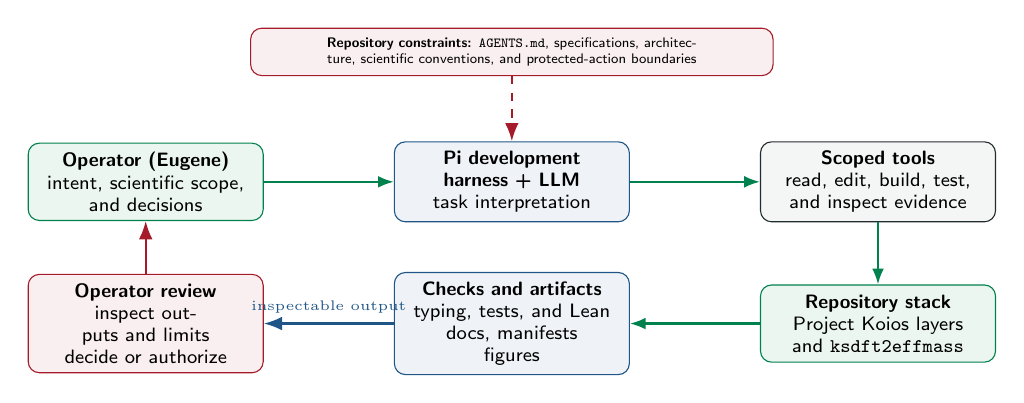
\begin{tikzpicture}[
      >=Latex,
      every node/.style={font=\sffamily\scriptsize,align=center},
      workflowstep/.style={rounded corners,minimum height=0.98cm,text width=2.75cm},
      flow/.style={-{Latex[length=2mm]},thick,dlsugreen}]
    \node[workflowstep,draw=dlsugreen,fill=dlsupalegreen] (operator) at (-4.65,0.80) {
      \textbf{Operator (Eugene)}\\intent, scientific scope,\\and decisions
    };
    \node[workflowstep,draw=resultblue,fill=resultblue!7] (pi) at (0,0.80) {
      \textbf{Pi development}\\\textbf{harness + LLM}\\task interpretation
    };
    \node[workflowstep,draw=charcoal,fill=lightgray] (tools) at (4.65,0.80) {
      \textbf{Scoped tools}\\read, edit, build, test,\\and inspect evidence
    };
    \node[workflowstep,draw=cautionred,fill=cautionred!7] (review) at (-4.65,-1.00) {
      \textbf{Operator review}\\inspect outputs and limits\\decide or authorize
    };
    \node[workflowstep,draw=resultblue,fill=resultblue!7] (checks) at (0,-1.00) {
      \textbf{Checks and artifacts}\\typing, tests, and Lean\\docs, manifests\\figures
    };
    \node[workflowstep,draw=dlsugreen,fill=dlsupalegreen] (repos) at (4.65,-1.00) {
      \textbf{Repository stack}\\Project Koios layers\\and \texttt{ksdft2effmass}
    };

    \draw[flow] (operator) -- (pi);
    \draw[flow] (pi) -- (tools);
    \draw[flow] (tools) -- (repos);
    \draw[flow] (repos) -- (checks);
    \draw[->,thick,resultblue] (checks) --
      node[above,font=\tiny] {inspectable output} (review);
    \draw[->,thick,cautionred] (review) -- (operator);

    \node[draw=cautionred,rounded corners,fill=cautionred!7,
      text width=6.4cm,font=\sffamily\tiny] (constraints) at (0,2.45) {
      \textbf{Repository constraints:} \texttt{AGENTS.md}, specifications,
      architecture, scientific conventions, and protected-action boundaries
    };
    \draw[->,dashed,thick,cautionred] (constraints) -- (pi);
  \end{tikzpicture}
  \vspace{0.20em}
  \begin{alertblock}{Human and formal checks constrain nondeterministic output}
    \centering\scriptsize
    Human-in-the-loop review, strong typing, tests, and selected Lean formalization make
    LLM-generated changes inspectable and auditable; they do not make the LLM
    deterministic. The operator retains scientific and protected-action authority, and
    passing software checks is not scientific validation.
  \end{alertblock}
\end{frame}

\begin{frame}{Strong types encode periodic and analysis spaces}
  \centering
  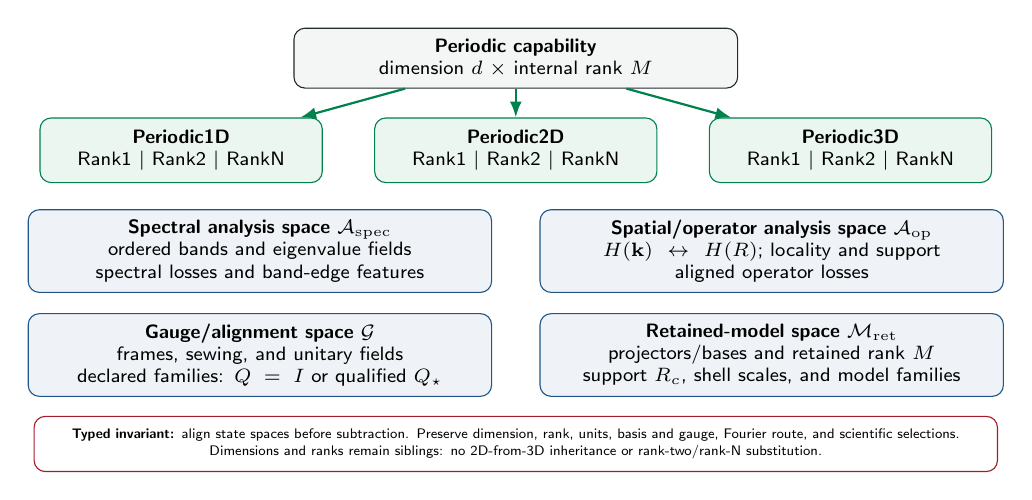
\begin{tikzpicture}[
      >=Latex,
      every node/.style={font=\sffamily\scriptsize,align=center},
      dimension/.style={draw=dlsugreen,rounded corners,fill=dlsupalegreen,
        minimum height=0.82cm,text width=3.35cm},
      analysis/.style={rounded corners,minimum height=1.05cm,text width=5.65cm},
      flow/.style={-{Latex[length=2mm]},thick,dlsugreen}]
    \node[draw=charcoal,rounded corners,fill=lightgray,
      minimum height=0.76cm,text width=5.4cm] (periodic) at (0,2.35) {
      \textbf{Periodic capability}\\dimension $d$ $\times$ internal rank $M$
    };
    \node[dimension] (d1) at (-4.25,1.18) {
      \textbf{Periodic1D}\\Rank1 $\mid$ Rank2 $\mid$ RankN
    };
    \node[dimension] (d2) at (0,1.18) {
      \textbf{Periodic2D}\\Rank1 $\mid$ Rank2 $\mid$ RankN
    };
    \node[dimension] (d3) at (4.25,1.18) {
      \textbf{Periodic3D}\\Rank1 $\mid$ Rank2 $\mid$ RankN
    };
    \draw[flow] (periodic) -- (d1);
    \draw[flow] (periodic) -- (d2);
    \draw[flow] (periodic) -- (d3);

    \node[analysis,draw=resultblue,fill=resultblue!7] (spectral) at (-3.25,-0.10) {
      \textbf{Spectral analysis space $\mathcal A_{\mathrm{spec}}$}\\
      ordered bands and eigenvalue fields\\spectral losses and band-edge features
    };
    \node[analysis,draw=resultblue,fill=resultblue!7] (spatial) at (3.25,-0.10) {
      \textbf{Spatial/operator analysis space $\mathcal A_{\mathrm{op}}$}\\
      $H(\mathbf k)\leftrightarrow H(R)$; locality and support\\aligned operator losses
    };
    \node[analysis,draw=resultblue,fill=resultblue!7] (gauge) at (-3.25,-1.42) {
      \textbf{Gauge/alignment space $\mathcal G$}\\
      frames, sewing, and unitary fields\\declared families: $Q=I$ or qualified $Q_\star$
    };
    \node[analysis,draw=resultblue,fill=resultblue!7] (retained) at (3.25,-1.42) {
      \textbf{Retained-model space $\mathcal M_{\mathrm{ret}}$}\\
      projectors/bases and retained rank $M$\\support $R_c$, shell scales, and model families
    };

    \node[draw=cautionred,rounded corners,fill=white,
      text width=12.0cm,minimum height=0.70cm,font=\sffamily\tiny] at (0,-2.55) {
      \textbf{Typed invariant:} align state spaces before subtraction. Preserve
      dimension, rank, units, basis and gauge, Fourier route, and scientific selections.\\
      Dimensions and ranks remain siblings: no 2D-from-3D inheritance or
      rank-two/rank-N substitution.
    };
  \end{tikzpicture}
\end{frame}

\section{Rank-two periodic theory}
{
\setbeamercolor{background canvas}{bg=dlsugreen}
\setbeamertemplate{footline}{}
\begin{frame}[plain]
  \centering
  \vfill
  
\includegraphics[width=.23\paperwidth]{assets/dlsu-wordmark-white.png}\par
  \vspace{0.8em}
  {\sffamily\bfseries\large\color{white!65}SECTION III\par}
  \vspace{0.25em}
  {\sffamily\bfseries\fontsize{30}{34}\selectfont\color{white}
  Rank-Two Periodic Theory\par}
  \vspace{0.4em}
  {\sffamily\large\color{white!85}
  Exact compatibility geometry in periodic dimension $d$\par}
  \vfill
\end{frame}
}

\begin{frame}{One band structure, two finite-range costs}
  \begin{columns}[T]
    \column{0.62\textwidth}
      \centering
      \includegraphics[width=\textwidth,height=0.73\textheight,keepaspectratio]
        {\calcroot/periodic1d/rank2/band-equivalence-versus-hopping-locality/analysis/development/figures/range-inflation-preview.pdf}
    \column{0.34\textwidth}
      \small
      \textbf{Before truncation:} identical bands by pointwise unitary similarity.
      \vspace{0.45em}

      Keep hoppings with $|R|\le R_c$ and find the first sampled $R_c$ reaching band
      error $\le10^{-8}\Eref$.
      \vspace{0.4em}

      \begin{block}{Smallest passing range}
        \centering
        \begin{tabular}{@{}lr@{}}
          Reference & $R_c=4$\\
          Rotated comparison & $R_c=10$
        \end{tabular}
      \end{block}
      \begin{alertblock}{Range cost}
        The rotated comparison needs six additional lattice steps.
      \end{alertblock}
  \end{columns}
\end{frame}


\begin{frame}{How identical bands produce different hopping locality}
  \begin{columns}[T]
    \column{0.47\textwidth}
      \begin{block}{Pointwise spectral equivalence}
        \[
          H'(\mathbf k)=U^\dagger(\mathbf k)H(\mathbf k)U(\mathbf k),
        \]
        \[
          \operatorname{spec}H'(\mathbf k)=\operatorname{spec}H(\mathbf k).
        \]
        A conventional band plot cannot distinguish the fields.
      \end{block}
    \column{0.47\textwidth}
      \begin{exampleblock}{Fourier representation}
        \[
          H'(\mathbf R)=\frac{1}{|\mathrm{BZ}|}
          \int_{\mathrm{BZ}}U^\dagger H U\,
          e^{-i\mathbf k\cdot\mathbf R}\,d\mathbf k.
        \]
        Momentum dependence in $U(\mathbf k)$ mixes Fourier modes and redistributes
        hopping power over $\mathbf R$.
      \end{exampleblock}
  \end{columns}
  \vspace{0.35em}
  \begin{columns}[T]
    \column{0.47\textwidth}
      \begin{block}{Under a gauge-aware identification}
        The two fields represent the same abstract operator, and the aligned residual
        vanishes.
      \end{block}
    \column{0.47\textwidth}
      \begin{alertblock}{Under one fixed identification}
        Matrix agreement and finite-range cost become additional requirements beyond
        band agreement.
      \end{alertblock}
  \end{columns}
  \vspace{0.12em}
  \begin{beamercolorbox}[rounded=true,sep=0.34em,wd=\textwidth]{block body example}
    \centering\small\bfseries\color{resultblue}
    Spectral equivalence does not determine finite-range locality. Under a fixed orbital
    identification, matrix agreement and locality become additional constraints.
  \end{beamercolorbox}
\end{frame}

\begin{frame}{From two error budgets to one compatibility question}
  \small
  \begin{columns}[T]
    \column{0.47\textwidth}
      \begin{block}{Spectral admissibility}
        \[
          \mathcal A_s(\tau_s)
          =\{p:L_{\mathrm{spec}}(p)\le\tau_s\}.
        \]
        Which candidates reproduce the bands within the declared spectral budget?
      \end{block}
    \column{0.47\textwidth}
      \begin{exampleblock}{Operator admissibility}
        \[
          \mathcal A_o(\tau_o)
          =\{p:L_{\mathrm{op},*}(p)\le\tau_o\}.
        \]
        Which candidates reproduce the represented operator after the allowed alignment?
      \end{exampleblock}
  \end{columns}
  \vspace{0.45em}
  {
  \setbeamercolor{block title}{fg=white,bg=charcoal}
  \setbeamercolor{block body}{fg=charcoal,bg=lightgray}
  \setbeamercolor{block title example}{fg=white,bg=charcoal}
  \setbeamercolor{block body example}{fg=charcoal,bg=lightgray}
  \setbeamercolor{block title alerted}{fg=white,bg=charcoal}
  \setbeamercolor{block body alerted}{fg=charcoal,bg=lightgray}
  \begin{columns}[T]
    \column{0.31\textwidth}
      \begin{block}{Joint match}
        \centering
        $\mathcal A_s\cap\mathcal A_o\ne\varnothing$\\[0.45em]
        One candidate passes both error budgets.
      \end{block}
    \column{0.31\textwidth}
      \begin{exampleblock}{Certified separation}
        \centering
        $\operatorname{dist}(\mathcal A_s,\mathcal A_o)>\rho_{\mathrm{sep}}$\\[0.45em]
        A verified bound rules out any candidate satisfying both budgets within the
        declared family.
      \end{exampleblock}
    \column{0.31\textwidth}
      \begin{alertblock}{Unresolved}
        \centering
        Neither statement is established.\\[0.45em]
        ``No witness found'' is not a separation proof.
      \end{alertblock}
  \end{columns}
  }
\end{frame}

\begin{frame}{Periodic-$d$ rank-two proof in arbitrary periodic dimension}
  \small
  \begin{beamercolorbox}[rounded=true,sep=0.30em,wd=\textwidth]{block body example}
    \centering
    $\mathbf q\in\mathbb T^d$, $\mathbf R\in\mathbb Z^d$;
    the periodic dimension $d$ is arbitrary, while the internal fiber rank remains two.
  \end{beamercolorbox}
  \vspace{0.15em}
  \begin{columns}[T]
    \column{0.42\textwidth}
      \begin{block}{Setup and admitted alignment}
        \scriptsize
        \[
          H(\mathbf q)=\bar E(\mathbf q)I_2+D(\mathbf q),
          \qquad \operatorname{tr}D=0,
        \]
        \[
          A(\mathbf q)=U(\mathbf q)^{\mathsf T}H(\mathbf q)U(\mathbf q),
          \qquad U(\mathbf q)\in SO(2),
        \]
        \[
          C_{s,\lambda}(\mathbf q)=\bar E I_2+s\Eref I_2+\lambda D.
        \]
        The comparison admits one global $R(\phi)\in SO(2)$, not the generating
        momentum-dependent field $U(\mathbf q)$.
      \end{block}
    \column{0.54\textwidth}
      \begin{exampleblock}{Four exact steps}
        \scriptsize
        \begin{enumerate}
          \setlength{\itemsep}{0.28em}
          \item $\langle I_2,D\rangle_F=0$ separates centroid and splitting errors.
          \item Conjugation by $R(\phi)$ rotates the real traceless coordinates through
            $2\phi$; maximizing one weighted correlation gives $\mu_{\max}$.
          \item Completing the square gives
            \[
              L_{\rm spec}^2=s^2+\kappa(\lambda-1)^2,
            \]
            \[
              L_{\rm op,*}^2=s^2+\kappa(\lambda-\mu_{\max})^2
              +\kappa(1-\mu_{\max}^2).
            \]
          \item Thresholding the two quadratics produces homothetic ellipses;
            periodic dimension enters only through the averages defining $\kappa$ and
            $\mu_{\max}$.
        \end{enumerate}
      \end{exampleblock}
  \end{columns}
  \vspace{0.08em}
  \begin{beamercolorbox}[rounded=true,sep=0.26em,wd=\textwidth]{block body alerted}
    \centering\scriptsize
    \textbf{Exact conclusion:}\quad
    $Q=\operatorname{diag}(1,\kappa)$,
    $c_s=(0,1)$,
    $c_o=(0,\mu_{\max})$, and the operator floor is
    $\kappa(1-\mu_{\max}^2)$.
    This is periodic-$d$ and internal-rank-two; the locality identity needs an additional
    flat-parent premise.
  \end{beamercolorbox}
\end{frame}

\begin{frame}{Constructing the admissible sets}
  \small
  \begin{beamercolorbox}[rounded=true,sep=0.20em,wd=\textwidth]{block body example}
    \centering\scriptsize
    Inputs: $(\kappa,\mu_{\max},\tau_s,\tau_o,\mathcal D)$ with
    $\mathcal D\subseteq\{(s,\lambda):\lambda\ge0\}$.
  \end{beamercolorbox}
  \vspace{0.10em}
  \begin{columns}[T]
    \column{0.44\textwidth}
      \begin{block}{1. Spectral admissible set}
        \tiny
        \[
          \mathcal A_s=\mathcal D\cap
          \{s^2+\kappa(\lambda-1)^2\le\tau_s^2\}.
        \]
        $c_s=(0,1)$ and $r_s=\tau_s$ in scaled coordinates.
      \end{block}
      \begin{exampleblock}{2. Operator floor and set}
        \tiny
        \[
          f_o=\kappa(1-\mu_{\max}^2).
        \]
        If $\tau_o^2<f_o$, then $\mathcal A_o=\varnothing$. Otherwise
        \[
          \begin{gathered}
            r_o^2=\tau_o^2-f_o,\\[-0.05em]
            \mathcal A_o=\mathcal D\cap
            \{s^2+\kappa(\lambda-\mu_{\max})^2\le r_o^2\}.
          \end{gathered}
        \]
      \end{exampleblock}
    \column{0.52\textwidth}
      \centering
      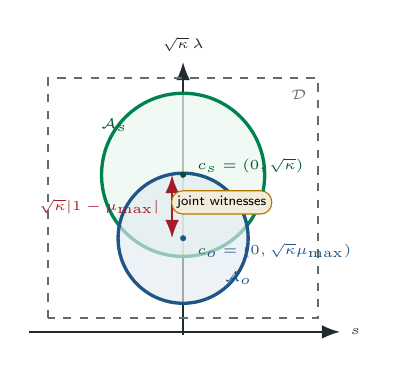
\begin{tikzpicture}[
          x=0.70cm,y=0.70cm,>=Latex,
          every node/.style={font=\sffamily\tiny}]
        \draw[->,thick,charcoal] (-2.8,-1.9) -- (2.85,-1.9) node[right] {$s$};
        \draw[->,thick,charcoal] (0,-1.95) -- (0,3.0)
          node[above] {$\sqrt\kappa\,\lambda$};
        \draw[dashed,thick,midgray] (-2.45,-1.65) rectangle (2.45,2.70);
        \node[anchor=north east,text=midgray] at (2.42,2.67) {$\mathcal D$};
        \draw[very thick,dlsugreen,fill=dlsupalegreen,fill opacity=0.72]
          (0,0.95) circle[radius=1.48];
        \draw[very thick,resultblue,fill=resultblue!12,fill opacity=0.66]
          (0,-0.20) circle[radius=1.18];
        \fill[dlsudarkgreen] (0,0.95) circle[radius=0.055];
        \fill[resultblue] (0,-0.20) circle[radius=0.055];
        \node[anchor=west,text=dlsudarkgreen] at (0.08,1.12)
          {$c_s=(0,\sqrt\kappa)$};
        \node[anchor=west,text=resultblue] at (0.08,-0.42)
          {$c_o=(0,\sqrt\kappa\mu_{\max})$};
        \draw[<->,cautionred,thick] (-0.20,-0.20) -- (-0.20,0.95);
        \node[anchor=east,text=cautionred,align=right] at (-0.25,0.38)
          {$\sqrt\kappa\lvert1-\mu_{\max}\rvert$};
        \node[text=dlsudarkgreen] at (-1.25,1.85) {$\mathcal A_s$};
        \node[text=resultblue] at (1.00,-0.92) {$\mathcal A_o$};
        \node[draw=warmgold,fill=warmgold!14,rounded corners,inner sep=2pt]
          at (0.70,0.45) {joint witnesses};
      \end{tikzpicture}

      {\tiny In $(s,\sqrt\kappa\lambda)$ coordinates, the ellipses become circles.}
  \end{columns}
  \vspace{0.05em}
  \centering
  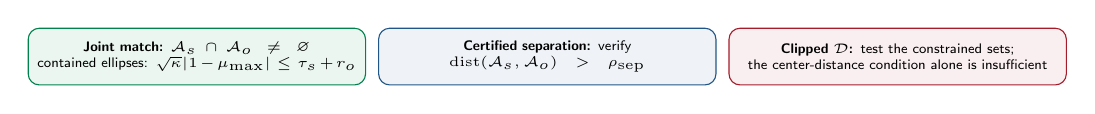
\begin{tikzpicture}[
      every node/.style={font=\sffamily\tiny,align=center},
      decision/.style={rounded corners,minimum height=0.72cm,text width=4.05cm}]
    \node[decision,draw=dlsugreen,fill=dlsupalegreen] (joint) at (-4.45,0)
      {\textbf{Joint match:} $\mathcal A_s\cap\mathcal A_o\ne\varnothing$\\
      contained ellipses: $\sqrt\kappa|1-\mu_{\max}|\le\tau_s+r_o$};
    \node[decision,draw=resultblue,fill=resultblue!7] (separate) at (0,0)
      {\textbf{Certified separation:} verify\\
      $\operatorname{dist}(\mathcal A_s,\mathcal A_o)>\rho_{\rm sep}$};
    \node[decision,draw=cautionred,fill=cautionred!7] (clipped) at (4.45,0)
      {\textbf{Clipped $\mathcal D$:} test the constrained sets;\\
      the center-distance condition alone is insufficient};
  \end{tikzpicture}
\end{frame}

\begin{frame}{Locality corollary: residual equals non-onsite power}
  \small
  \begin{beamercolorbox}[rounded=true,sep=0.24em,wd=\textwidth]{block body example}
    \centering
    {\sffamily\bfseries\color{resultblue}Exact flat-parent result}\par
    \vspace{0.18em}
    {\normalsize\color{charcoal}$\displaystyle
      \inf_{s,\lambda\ge0,\phi}L_{\mathrm{op},\phi}^2
      =\kappa(1-\mu_{\max}^2)
      =\frac{1}{2\Eref^2}
       \sum_{\mathbf R\ne\mathbf0}\norm{B_{\mathbf R}}_F^2$}\par
    \vspace{0.20em}
    {\scriptsize Best global $SO(2)$ fit $\rightarrow B_{\mathbf0}$;
    Parseval remainder $\rightarrow$ all $\mathbf R\ne\mathbf0$ blocks.}
  \end{beamercolorbox}
  \vspace{0.12em}
  \begin{columns}[T]
    \column{0.63\textwidth}
      \centering
      {\sffamily\bfseries\color{dlsudarkgreen}$d=1$ plotted illustration}\par
      \vspace{0.08em}
      \includegraphics[width=\textwidth,height=0.35\textheight,keepaspectratio]
        {\calcroot/periodic1d/rank2/band-equivalence-versus-hopping-locality/protocol/figures/storyboard/01-analytic-benchmark.pdf}
    \column{0.33\textwidth}
      \begin{block}{Periodic-$d$ sine family}
        \scriptsize
        \[
          \begin{gathered}
            U_a^{(d)}(\mathbf q)=R\!\left[
            \frac a d\sum_{j=1}^{d}\sin(2\pi q_j)\right],\\[0.1em]
            \mu_{\max}^{(d)}(a)=J_0(2a/d)^d.
          \end{gathered}
        \]
      \end{block}
  \end{columns}
\end{frame}

\section{Rank-10 silicon}
{
\setbeamercolor{background canvas}{bg=dlsugreen}
\setbeamertemplate{footline}{}
\begin{frame}[plain]
  \centering
  \vfill
  
\includegraphics[width=.23\paperwidth]{assets/dlsu-wordmark-white.png}\par
  \vspace{0.8em}
  {\sffamily\bfseries\large\color{white!65}SECTION IV\par}
  \vspace{0.25em}
  {\sffamily\bfseries\fontsize{30}{34}\selectfont\color{white}
  Rank-10 Silicon\par}
  \vspace{0.4em}
  {\sffamily\large\color{white!85}
  Source-relative Wannier reduction and band-edge diagnostics\par}
  \vspace{0.35em}
  {\sffamily\small\color{white!70}
  Exact finite separation extends to every retained dimension $N\ge2$;\\
  the two-point construction and its limitations are in backup.\par}
  \vfill
\end{frame}
}

\begin{frame}{From DFT to Wannier90 to this reduction study}
  \centering
  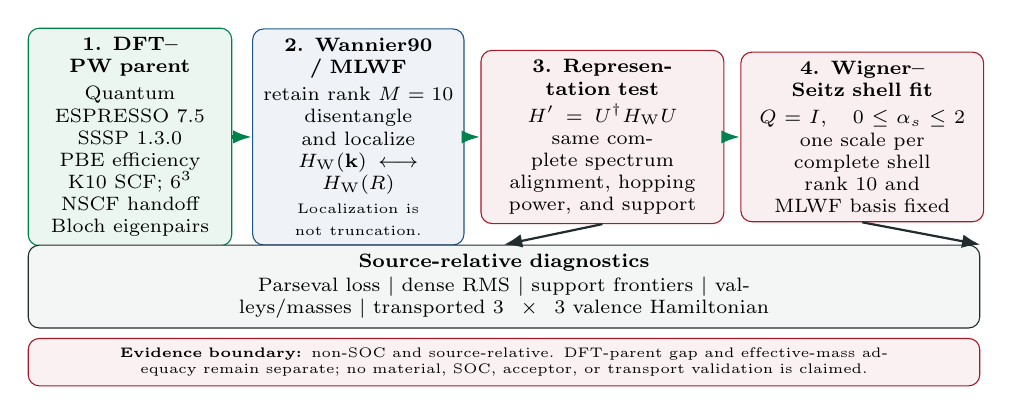
\begin{tikzpicture}[
      >=Latex,
      every node/.style={font=\sffamily,align=center},
      stage/.style={rounded corners,minimum height=1.82cm,font=\scriptsize},
      flow/.style={-{Latex[length=2.4mm,width=1.7mm]},very thick,dlsugreen}]

    \node[stage,draw=dlsugreen,fill=dlsupalegreen,text width=2.35cm]
      (dft) at (-4.75,1.18) {
      \textbf{1. DFT--PW parent}\\[0.22em]
      Quantum ESPRESSO 7.5\\
      SSSP 1.3.0 PBE efficiency\\
      K10 SCF; $6^3$ NSCF handoff\\
      Bloch eigenpairs
    };

    \node[stage,draw=resultblue,fill=resultblue!7,text width=2.45cm]
      (wannier) at (-1.85,1.18) {
      \textbf{2. Wannier90 / MLWF}\\[0.22em]
      retain rank $M=10$\\
      disentangle and localize\\
      $H_{\mathrm W}(\mathbf k)\longleftrightarrow H_{\mathrm W}(R)$\\[0.10em]
      {\tiny Localization is not truncation.}
    };

    \node[stage,draw=cautionred,fill=cautionred!7,text width=2.85cm]
      (gauge) at (1.25,1.18) {
      \textbf{3. Representation test}\\[0.22em]
      $H'=U^\dagger H_{\mathrm W}U$\\
      same complete spectrum\\
      alignment, hopping power, and support
    };

    \node[stage,draw=cautionred,fill=cautionred!7,text width=2.85cm]
      (fit) at (4.55,1.18) {
      \textbf{4. Wigner--Seitz shell fit}\\[0.22em]
      $Q=I,\quad0\leq\alpha_s\leq2$\\
      one scale per complete shell\\
      rank 10 and MLWF basis fixed
    };

    \draw[flow] (dft) -- (wannier);
    \draw[flow] (wannier) -- (gauge);
    \draw[flow] (gauge) -- (fit);

    \node[draw=charcoal,rounded corners,fill=lightgray,
      minimum height=0.84cm,text width=11.85cm,font=\scriptsize] (diagnostics) at (0,-0.72) {
      \textbf{Source-relative diagnostics}\\[0.08em]
      Parseval loss $\mid$ dense RMS $\mid$ support frontiers $\mid$ valleys/masses
      $\mid$ transported $3\times3$ valence Hamiltonian
    };
    \draw[->,thick,charcoal] (gauge.south) -- (diagnostics.north);
    \draw[->,thick,charcoal] (fit.south) -- (diagnostics.north east);

    \node[draw=cautionred,rounded corners,fill=cautionred!6,
      minimum height=0.55cm,text width=11.85cm,font=\tiny] at (0,-1.68) {
      \textbf{Evidence boundary:} non-SOC and source-relative. DFT-parent gap and
      effective-mass adequacy remain separate; no material, SOC, acceptor, or transport
      validation is claimed.
    };
  \end{tikzpicture}
\end{frame}

\begin{frame}{Can the mechanism survive in rank 10?}
  \begin{columns}[T]
    \column{0.57\textwidth}
      \centering
      \includegraphics[width=\textwidth,height=0.72\textheight,keepaspectratio]
        {\calcroot/Si/bulk/simulations/evidence/sssp-1.3.0-pbe-efficiency-qe-7.5-accepted-s1-parent-bands-l-gamma-x-gamma-b20/figures/parent-dft-band-diagram.pdf}
    \column{0.39\textwidth}
      \small
      \begin{block}{Source}
        Non-SOC rank-10 $C6$--$B20$--$W21$ silicon Wannier Hamiltonian on a $6^3$
        construction mesh.
      \end{block}
      \begin{exampleblock}{Test}
        Apply a frozen momentum-dependent Givens circuit and compare alignment,
        Fourier power, support, interpolation, and band-edge consequences.
      \end{exampleblock}
      \boundary{The source fails separate DFT-parent gap/effective-mass targets.}
  \end{columns}
\end{frame}

\begin{frame}{A unitary change of frame alters locality, not the spectrum}
  \begin{columns}[T]
    \column{0.66\textwidth}
      \centering
      \includegraphics[width=\textwidth,height=0.70\textheight,keepaspectratio,
        trim=0 42 0 0,clip]
        {\calcroot/Si/bulk/analysis/c6-b20-w21-gauge-alignment-locality/figures/alignment-invariance.pdf}
    \column{0.30\textwidth}
      \scriptsize
      \begin{exampleblock}{Spectrum check}
        Maximum sorted-spectrum difference:\\[0.15em]
        \centering\bfseries $3.20\times10^{-14}$ eV.
      \end{exampleblock}
      \begin{block}{Non-onsite power}
        \centering\bfseries
        $20.7574\rightarrow21.5057$ eV$^2$/retained state.
      \end{block}
  \end{columns}
\end{frame}

\begin{frame}{Support--error frontiers depend on representation}
  \begin{columns}[T,onlytextwidth]
    \column{0.69\textwidth}
      \centering
      \includegraphics[width=\textwidth,height=0.73\textheight,keepaspectratio,
        trim=18 44 18 80,clip]
        {\calcroot/Si/bulk/analysis/c6-b20-w21-gauge-alignment-locality/figures/pareto-support-error-frontiers.pdf}
    \column{0.28\textwidth}
      \begin{block}{Support--error tradeoff}
        \scriptsize
        Horizontal position is the number of retained complete rank-10 lattice blocks;
        vertical position is total error. Lower and farther left is better.
      \end{block}
      \begin{exampleblock}{Representation effect}
        \scriptsize
        The non-dominated observed supports shift in the matrix and ordered-spectrum
        channels after the unitary change of frame.
      \end{exampleblock}
      \begin{beamercolorbox}[rounded=true,sep=0.45em,wd=\textwidth]{block body example}
        \centering\scriptsize\bfseries\color{resultblue}
        The complete spectrum is unchanged, but the finite-support tradeoff moves.
      \end{beamercolorbox}
      \vspace{0.35em}
      {\tiny\color{cautionred}\textbf{Boundary.}
      These are discrete finite-inventory frontiers, not certified global optima or
      infeasibility results.\par}
  \end{columns}
\end{frame}

\begin{frame}{Wigner--Seitz deletion versus shell fitting}
  \begin{columns}[T]
    \column{0.49\textwidth}
      \centering
      \includegraphics[width=\textwidth,height=0.53\textheight,keepaspectratio,
        trim=0 0 0 76,clip]
        {\calcroot/Si/bulk/analysis/c6-b20-w21-tau1-tau2-posthoc-exploration/figures-v5/single-witness-surface.pdf}
      \scriptsize Literal complete Wigner--Seitz shell deletion
    \column{0.49\textwidth}
      \centering
      \includegraphics[width=\textwidth,height=0.53\textheight,keepaspectratio,
        trim=0 0 0 76,clip]
        {\calcroot/Si/bulk/analysis/c6-b20-w21-refitted-ws-shell-witness-posthoc/figures-v2/single-refitted-witness-surface.pdf}
      \scriptsize Wigner--Seitz shell-scale fitting, $0\le\alpha_s\le2$
  \end{columns}
  \vspace{0.10em}
  \begin{itemize}
    \small
    \setlength{\itemsep}{0.08em}
    \item The bounded multistart search produced 444 converged optimization witnesses;
      convergence does not by itself establish feasibility.
    \item Gray regions mark ``no witness found''; they do not certify global
      infeasibility.
    \item H-shell-16 retains $371/383=96.9\%$ of representatives: near-full support,
      not a compact Hamiltonian.
  \end{itemize}
\end{frame}

\begin{frame}{Fit-sample error understates dense and integrated error}
  \begin{columns}[T,onlytextwidth]
    \column{0.63\textwidth}
      \begin{block}{Spectral RMS: 408 points $\rightarrow$ dense $32^3$ mesh}
        \centering\small
        \begin{tabular}{@{}lrrr@{}}
          \toprule
          Model & Fit (eV) & Dense (eV) & Increase\\
          \midrule
          H-shell-05 & 0.07242 & 0.18196 & $2.51\times$\\
          H-shell-10 & 0.01320 & 0.02785 & $2.11\times$\\
          H-shell-16 & 0.000404 & 0.000657 & $1.62\times$\\
          \bottomrule
        \end{tabular}
      \end{block}
      \begin{exampleblock}{Operator RMS: 408 points $\rightarrow$ Parseval integral}
        \centering\small
        \begin{tabular}{@{}lrrr@{}}
          \toprule
          Model & Fit (eV) & Parseval (eV) & Increase\\
          \midrule
          H-shell-05 & 0.12814 & 0.26004 & $2.03\times$\\
          H-shell-10 & 0.03229 & 0.05956 & $1.84\times$\\
          H-shell-16 & 0.001394 & 0.001747 & $1.25\times$\\
          \bottomrule
        \end{tabular}
      \end{exampleblock}

    \column{0.34\textwidth}
      \begin{block}{What changes off the fit set?}
        \scriptsize
        Every reported error increases when evaluated on a denser or integrated domain.
        The 408 optimization points therefore understate broader source-relative error.
      \end{block}
      \begin{exampleblock}{Independent arithmetic check}
        \scriptsize
        Directly sampled operator RMS and exact Parseval evaluation agree to
        $5.56\times10^{-17}$ eV when evaluated under the same convention.
      \end{exampleblock}
      \begin{beamercolorbox}[rounded=true,sep=0.48em,wd=\textwidth]{block body example}
        \centering\small\bfseries\color{resultblue}
        Fit loss, dense interpolation, and band-edge fidelity are distinct tests.
      \end{beamercolorbox}
  \end{columns}
\end{frame}

\begin{frame}{A small spectral RMS can hide a large mass error}
  \centering
  \includegraphics[width=0.97\textwidth,height=0.56\textheight,keepaspectratio]
    {\calcroot/Si/bulk/analysis/c6-b20-w21-wannier-only-comprehensive-band-edge/figures-v3/derived-electron-mass-fidelity.pdf}
  \vspace{0.12em}
  \begin{beamercolorbox}[rounded=true,sep=0.42em,wd=0.96\textwidth]{block body alerted}
    \centering
    {\large\bfseries H-shell-10: spectral RMS $=0.02785$ eV, yet the maximum principal
    electron-mass change is $53.2\%$.}\par
    \vspace{0.12em}
    {\scriptsize Context: H-shell-05 changes by $67.7\%$; H-shell-16 by $2.54\%$.
    A good-looking dense-band RMS is not a band-edge certificate.}
  \end{beamercolorbox}
\end{frame}

\begin{frame}{Valence degeneracy is an internal-fidelity test}
  \centering
  \includegraphics[width=0.96\textwidth,height=0.57\textheight,keepaspectratio]
    {\calcroot/Si/bulk/analysis/c6-b20-w21-wannier-only-comprehensive-band-edge/figures-v3/gamma-valence-cluster-fidelity.pdf}
  \vspace{0.10em}
  \begin{beamercolorbox}[rounded=true,sep=0.38em,wd=0.96\textwidth]{block body example}
    \centering
    {\bfseries Gamma splitting:}
    source $0.025$ meV $\mid$ H-shell-05 $102.2$ meV $\mid$
    H-shell-10 $54.8$ meV $\mid$ H-shell-16 $2.50$ meV.\\[0.18em]
    {\scriptsize Subspace overlap can remain good while the internal Hamiltonian of the
    nearly degenerate cluster is substantially distorted.}
  \end{beamercolorbox}
\end{frame}

\begin{frame}{The correct valence object is matrix-valued}
  \centering
  \begin{beamercolorbox}[rounded=true,sep=0.20em,wd=0.96\textwidth]{block body example}
    \centering\scriptsize
    Transport the three-band cluster into one common coefficient space:
    $\displaystyle H_{\mathrm{eff}}(\mathbf q)=H_{\mathrm{eff}}(0)
    +\sum_iq_iA_i+\sum_{ij}q_iq_jB_{ij}+O(\norm{\mathbf q}^3)$.
    For direction $\hat{\mathbf n}$, the eigenvalues of
    $\displaystyle 2\sum_{ij}n_in_jB_{ij}$ are basis-invariant curvature channels.
  \end{beamercolorbox}
  \vspace{0.10em}
  \includegraphics[width=0.97\textwidth,height=0.47\textheight,keepaspectratio]
    {\calcroot/Si/bulk/analysis/c6-b20-w21-wannier-only-comprehensive-band-edge/figures-v3/multiband-valence-fidelity-summary.pdf}
  \vspace{0.08em}
  \begin{beamercolorbox}[rounded=true,sep=0.22em,wd=0.96\textwidth]{block body alerted}
    \centering\bfseries
    Preserve both the transported subspace and its internal $3\times3$ quadratic Hamiltonian.\\[-0.02em]
    {\scriptsize Non-SOC orbital curvature channels---not physical heavy-hole,
    light-hole, or split-off masses.}
  \end{beamercolorbox}
\end{frame}

\begin{frame}{The source can fail upstream and still teach us downstream}
  \begin{columns}[T,onlytextwidth]
    \column{0.49\textwidth}
      \begin{block}{Deliberate numerical stress test}
        \scriptsize
        The DFT-derived rank-10 Wannier operator was subjected to severe complete-shell
        deletion and shell-scale fitting to expose representation, truncation, and
        feature-fidelity errors.
      \end{block}
      \begin{exampleblock}{Mesh roles must remain separate}
        \scriptsize
        The accepted parent SCF uses a Gamma-centered K10 mesh and the active Wannier
        source uses a $6^3$ construction mesh. The $12^3$, $20^3$, and $32^3$ meshes are
        post-fit interpolation tests---not a $12^3$ parent DFT calculation that was
        reduced.
      \end{exampleblock}
      \begin{alertblock}{Source adequacy}
        \scriptsize
        The full source fails separate DFT-parent gap and most effective-mass targets;
        no reduction can repair that upstream discrepancy.
      \end{alertblock}

    \column{0.48\textwidth}
      \begin{block}{Physics scope}
        \scriptsize
        The calculations are non-SOC. They do not support physical heavy-hole,
        light-hole, split-off, acceptor, spin-dependent, or transport claims.
      \end{block}
      \begin{alertblock}{Certificate scope}
        \scriptsize
        Lean-based certificate checking is not implemented for the silicon admissible
        sets. Bounded multistart optimization supplies constructive witnesses only;
        identified valleys and ``no witness found'' outcomes are not global certificates.
      \end{alertblock}
      \begin{exampleblock}{Mechanism still testable}
        \scriptsize
        The source remains sufficient to test how a frozen unitary change of frame and
        complete-shell reduction affect alignment, Fourier power, support, and
        source-relative fidelity.
      \end{exampleblock}
  \end{columns}
\end{frame}

\section{Conclusion}
{
\setbeamercolor{background canvas}{bg=dlsugreen}
\setbeamertemplate{footline}{}
\begin{frame}[plain]
  \centering
  \vfill
  
\includegraphics[width=.23\paperwidth]{assets/dlsu-wordmark-white.png}\par
  \vspace{0.8em}
  {\sffamily\bfseries\large\color{white!65}SECTION V\par}
  \vspace{0.25em}
  {\sffamily\bfseries\fontsize{30}{34}\selectfont\color{white}Conclusion\par}
  \vspace{0.4em}
  {\sffamily\large\color{white!85}
  Scientific boundaries, take-home messages, and next steps\par}
  \vfill
\end{frame}
}

\begin{frame}{Take-home messages}
  \large
  \begin{enumerate}
    \item \textbf{Bands do not determine locality.}
    \item \textbf{Alignment is part of the model definition.}
    \item \textbf{Fit loss, dense interpolation, and band-edge fidelity are different tests.}
    \item \textbf{Near-full support is not a compact reduction.}
    \item \textbf{Source-relative fidelity is not physical validation.}
  \end{enumerate}
  \vspace{0.55em}
  \takeaway{A reduced Hamiltonian should be accepted against the operator and observables
  it is intended to reproduce---not against a band plot alone.}
\end{frame}

\begin{frame}{What comes next: operator reduction beyond silicon}
  \small
  \begin{columns}[T,onlytextwidth]
    \column{0.49\textwidth}
      \begin{block}{Wigner--Seitz $\rightarrow$ Slater--Koster}
        \scriptsize
        Build a qualified common-space map from the retained Wigner--Seitz hopping
        representation to an orbital-parametric Slater--Koster basis, then test spectral
        and operator admissibility together.
      \end{block}
      \begin{block}{Doping beyond effective mass}
        \scriptsize
        Represent dopant potentials and host--defect coupling as reduced operators,
        retaining screening, symmetry, localization, finite-domain effects, and
        provenance rather than only effective-mass tensors.
      \end{block}
    \column{0.49\textwidth}
      \begin{exampleblock}{Electron--phonon coupling operators}
        \scriptsize
        Develop an EPL-like reduction workflow for coupling operators with aligned
        electronic and phonon state spaces; keep gauge, interpolation, truncation, and
        observable fidelity as separate error channels.
      \end{exampleblock}
      \begin{exampleblock}{Conjugated donor--acceptor polymers}
        \scriptsize
        Start from the DFT--O orbital representation, construct aligned local operators
        for donor--acceptor systems, and test spectral/operator compatibility before
        finite-range reduction.
      \end{exampleblock}
  \end{columns}
\end{frame}

\begin{frame}[plain]
  \centering
  \vfill
  
\includegraphics[width=.30\paperwidth]{assets/dlsu-wordmark-green.png}\par
  \vspace{1.0em}
  {\usebeamerfont{title}\color{dlsudarkgreen}Thank you.\par}
  \vspace{0.7em}
  {\large Questions?\par}
  \vspace{1.0em}
  {\small\color{midgray}Band equivalence is not locality.}
  \vfill
\end{frame}

% -----------------------------------------------------------------------------
% Backup material: not counted in the main slide total.
% -----------------------------------------------------------------------------
\appendix

\begin{frame}{Backup: evidence status}
  \scriptsize
  \begin{tabular}{@{}p{0.22\textwidth}p{0.32\textwidth}p{0.38\textwidth}@{}}
    \toprule
    Layer & Strongest retained statement & Boundary \\
    \midrule
    Analytic rank two & Exact loss geometry and residual--tail identity & Restricted theorem assumptions \\
    Controlled rank two & Sampled range inflation from $4$ to $10$ & Declared unitary field, mesh, target, and cutoff inventory \\
    Rank-10 silicon & Spectrum invariant; locality and finite-support behavior change & Producer checked; not independently reconstructed \\
    Convention audit & Six-valley formulas and exact size-six mode inventory agree & No fields, valleys, Hessians, or removed coefficients reconstructed \\
    DFT context & Accepted-S1 path and revealed 408-point adequacy audit & Context/development evidence, not material validation \\
    \bottomrule
  \end{tabular}
\end{frame}

\begin{frame}{Backup: rank-two assumptions}
  \small
  The residual--non-onsite-power identity assumes:
  \begin{itemize}
    \item a flat, traceless, real-symmetric $2\times2$ parent;
    \item a generating unitary field in the same real-rotation orbit;
    \item one global real-rotation alignment and a nonnegative scale;
    \item normalized continuum measure or uniform finite weights;
    \item matched Fourier normalization.
  \end{itemize}
  The invariant correlation term is nonnegative, so the reported scale optimum is not
  clipped. For a different orbit with negative maximal correlation, minimization over
  $\lambda\ge0$ would stop at $\lambda=0$.
\end{frame}

\begin{frame}{Backup: controlled numerical protocol}
  \small
  \begin{itemize}
    \item finite-range four-state parent; retained lower rank-two projector;
    \item parallel transport with periodic sewing and overlap-rank gates;
    \item centered construction meshes up to $N=512$;
    \item shifted, disjoint evaluation mesh with $N_{\mathrm{eval}}=1025$;
    \item ordinary-lattice cutoffs $R_c=0,\ldots,16$;
    \item first-passing decision uses maximum ordered-band error;
    \item interpolation, truncation, and total finite-model errors retained separately.
  \end{itemize}
\end{frame}

\begin{frame}{Backup: size-six Fourier conversion}
  \small
  \begin{columns}[T]
    \column{0.52\textwidth}
      Cyclic inventory:
      \[
        \{-3,-2,-1,0,1,2\}^3,\qquad216\ \text{records}.
      \]
      Remove every record touching $-3=-N/2$:
      \[
        91\ \text{removed},\qquad125\ \text{retained}.
      \]
      Retained modes map identically to $\{-2,-1,0,1,2\}^3$.
    \column{0.44\textwidth}
      \begin{exampleblock}{Independent audit}
        FCC metric labels agree; maximum radius discrepancy is
        $3.55\times10^{-15}$~\AA.
      \end{exampleblock}
      \begin{alertblock}{Unavailable}
        The 216 cyclic matrices and removed-mode coefficient power were not retained and
        were not reconstructed.
      \end{alertblock}
  \end{columns}
\end{frame}

\begin{frame}{Backup: six-valley mass conventions}
  \small
  For valley mass tensor $M_v$:
  \begin{align*}
    m_{\mathrm{DOS},1v}&=\det(M_v)^{1/3},&
    m_{\mathrm{cond},1v}&=\frac{3}{\operatorname{tr}(M_v^{-1})},\\
    m_{\mathrm{DOS},6v}&=\left[\sum_v\sqrt{\det M_v}\right]^{2/3},&
    m_{\mathrm{cond},6v}&=\frac{3}{\operatorname{tr}[(1/6)\sum_vM_v^{-1}]}.
  \end{align*}
  \begin{exampleblock}{Independent arithmetic}
    Maximum difference from separate NumPy calculations:
    $6.22\times10^{-15}$.
  \end{exampleblock}
  The conductivity convention averages inverse-mass tensors, not scalar conductivity masses.
\end{frame}

\begin{frame}{Backup: Slater--Koster is not the active fit}
  \small
  \begin{columns}[T]
    \column{0.48\textwidth}
      \begin{block}{Active reduction family}
        The reported fit rescales complete native Wigner--Seitz shells,
        \[
          0\le\alpha_s\le2,
        \]
        while preserving the rank-10 Wannier basis and all matrices within each shell.
      \end{block}
    \column{0.48\textwidth}
      \begin{alertblock}{Separate Slater--Koster path}
        A common-space gate for a joint orbital-aligned Slater--Koster fit was rank
        deficient (rank 9) at Gamma and one additional point, so no joint fit was run.
      \end{alertblock}
  \end{columns}
  \vspace{0.4em}
  This does not establish a Slater--Koster impossibility theorem; it only excludes that
  unqualified route from the active results \cite{slater1954,vogl1983}.
\end{frame}

\begin{frame}{Backup: ordered valence branches are window sensitive}
  \centering
  \includegraphics[width=0.91\textwidth,height=0.76\textheight,keepaspectratio]
    {\calcroot/Si/bulk/analysis/c6-b20-w21-wannier-only-comprehensive-band-edge/figures-v3/directional-valence-mass-sensitivity.pdf}
  \vspace{-0.25em}
  {\scriptsize Missing curves correspond to positive fitted curvature, for which no apparent hole mass is reported.}
\end{frame}

\begin{frame}{Backup: reproducibility boundary}
  \small
  Retained calculation packages contain requests, source identities, producer scripts,
  machine-readable results, figures, manifests, and execution records.
  \begin{alertblock}{Current limitation}
    No public repository URL or DOI yet contains the complete authenticated source data
    and independent reconstruction environment. Local paths and hashes are audit anchors,
    not a public reproduction package.
  \end{alertblock}
  No new QE, Wannier90, Hamiltonian construction, optimization, valley search, or Hessian
  calculation was performed to prepare these slides.
\end{frame}

\begin{frame}{Backup: exact separation for every retained dimension}
  \scriptsize
  \begin{beamercolorbox}[rounded=true,sep=0.38em,wd=\textwidth]{block body example}
    \centering
    For $N\ge2$, let $A_N=\operatorname{diag}(\varepsilon_0<\cdots<\varepsilon_{N-1})$
    on $K=\mathbb Z/2\mathbb Z$, with $G_{01}$ swapping the first two coordinates.\\[0.18em]
    $U(0)=I,\quad U(1)=G_{01},\quad B(k)=U(k)^\dagger A_NU(k)$.
  \end{beamercolorbox}
  \vspace{0.15em}
  \begin{columns}[T,onlytextwidth]
    \column{0.32\textwidth}
      \begin{block}{Pointwise spectrum}
        \centering\vspace{0.22em}
        $\operatorname{spec}_{\mathbb C}B(k)=\operatorname{spec}_{\mathbb C}A_N$.
        \vspace{0.22em}
      \end{block}
    \column{0.32\textwidth}
      \begin{alertblock}{Truncation does not commute}
        \centering\vspace{0.22em}
        $T_0[U^\dagger H_AU]\ne U^\dagger T_0[H_A]U$.
        \vspace{0.22em}
      \end{alertblock}
    \column{0.32\textwidth}
      \begin{exampleblock}{Positive omitted power}
        \centering\vspace{0.22em}
        $P_{\mathrm{omit}}(\widehat B;\{0\})>0$.
        \vspace{0.22em}
      \end{exampleblock}
  \end{columns}
  \vspace{0.05em}
  \begin{columns}[T,onlytextwidth]
    \column{0.48\textwidth}
      \begin{block}{Generic exact result}
        If a finite-dimensional operator satisfies $A\ne G^\dagger AG$, the same
        two-point construction gives all three conclusions with one common witness.
      \end{block}
    \column{0.48\textwidth}
      \begin{block}{Concrete rank-$N$ witness}
        The analytic parent contains all $N$ strictly ordered retained energies. This is
        retained-space dimension $N$, not algebraic matrix rank or a rank-two embedding.
      \end{block}
  \end{columns}
  \begin{alertblock}{Exact scope and current status}
    \tiny
    $N$ is retained-space dimension, not algebraic matrix rank. This is a minimal
    $\mathbb Z/2\mathbb Z$ witness with spectrum equality as complex sets; it proves no
    realistic-mesh, runtime-FFT, continuum-locality, or material statement. Targeted Lean
    compilation and the no-admission scan pass in a development worktree; promotion and a
    frozen audit remain pending. IDs: BG-FOURIER-GAUGE-THM-013/014.
  \end{alertblock}
\end{frame}

\begin{frame}[allowframebreaks]{Backup: references}
  \tiny
  \nocite{
    hohenberg1964,kohn1965,perdew1996,giannozzi2009,giannozzi2017,
    giannozzi2020,hamann2013,vansetten2018,monkhorst1976,
    wannier1937,kohn1959,desCloizeaux1964,marzari1997,souza2001,marzari2012,
    mostofi2008,pizzi2020,mustafa2015,cances2017,damle2018,vitale2020,brouder2007,
    bjork1973,schonemann1966,higham1986,davis1970,hornJohnson2013,
    golubVanLoan2013,shankar1994,teschl2014,strikwerda2004,
    slater1954,vogl1983,starrost1996,stiles1997,klimeck2000,
    boykinKlimeckOyafuso2004,wangEtAl2021,zhangEtAl2022,schwadeEtAl2026,
    luttingerKohn1955,kittel2004,yuCardona2010,rubel2021effectiveMass,
    feshbach1958,feshbach1962,lowdin1962,bravyi2011,benzi2013,prodanKohn2005,
    rudin1976,milaneseEtAl1996,neumaier2004,mooreKearfottCloud2009,
    kosterSlater1954impurity,kohnLuttinger1955donor,nakamuraTadano2021,
    freysoldt2014,sandve2013,coveney2021reliability,ye2021uqPatterns,
    bect2021discretization,mathlib2020}
  \printbibliography[heading=none]
\end{frame}

\end{document}
